\section{Background}\label{sec:background}

\textbf{The retina.}
In vertebrates, the retina is part of the central nervous system. It consists
of just a few layers of neurons, each with a distinct role in processing visual
information \ref*{fig:retina_structure}. ADD FIGURE ON THE STRUCTURE OF THE RETINA

\begin{figure}[h]
    \centering
    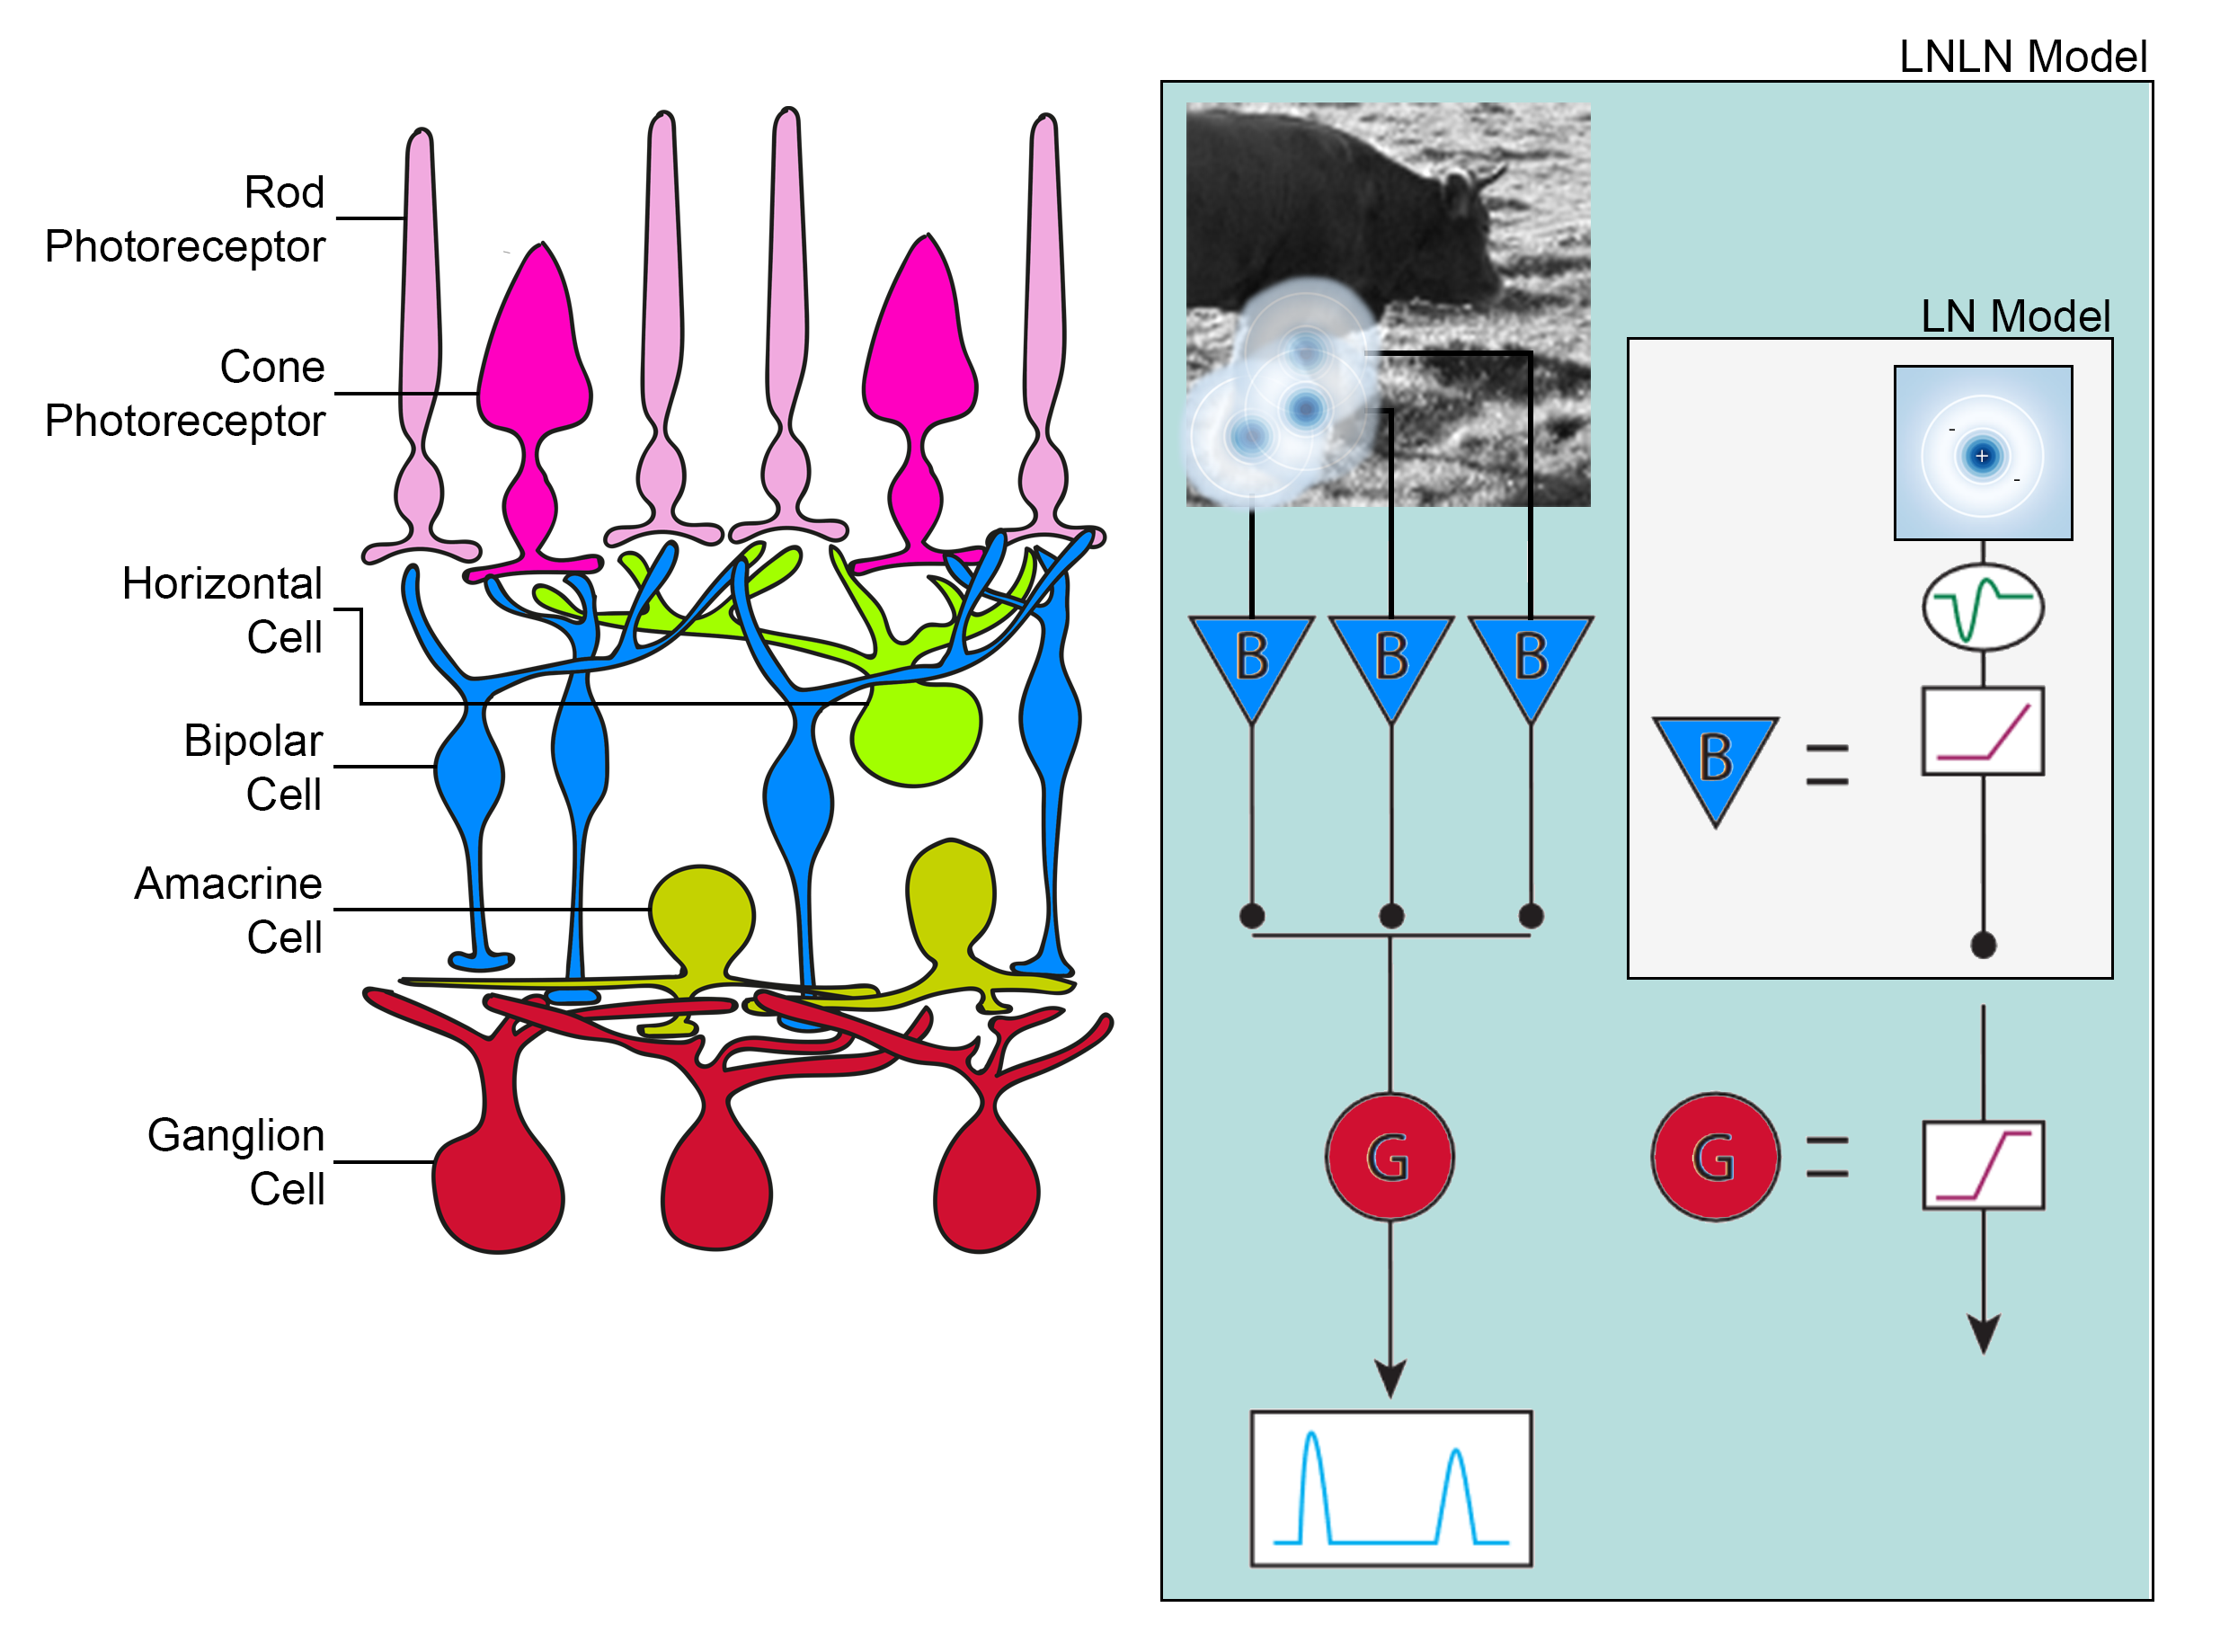
\includegraphics[width=0.8\textwidth]{pics/RetinaAnatToFunction.png}
    \caption{The structure of the retina.}
    \label{fig:retina_structure}
\end{figure}



At its forefront are photosensitive neurons known as photoreceptors, which
serve as the initial light sensors within this neural network. ADD ABOUT CONES
AND RODS

These photoreceptors stimulate bipolar cells, a diverse group comprising 15-20
anatomical
distinct types in the mouse. They all exhibit unique
responses to visual stimuli, with an even larger functional complexity than
anatomical diveristy. % Functional/genetic/anatomical types?

The bipolar cells, in turn, excite retinal ganglion cells (RGC), the final
relay in the
chain, which then transmit the pre-processed visual data to the rest of the
brain
via the optic nerve. RGC of the same type are described as sharing the same
physiology morphology,
intra-retinal connectivity, retinal mosaic and genetic markers. It is not yet
known if such biological markers are enough to define the variety of functional
output channels of the retina. According to Baden and co-worker, there should
be at least 32 different RGC
functional types \citep*{baden_functional_2016}. An example of functional
diversity in the RGC groups is their preference for local light increase and/or
decrease. They are respectively refered as ON, OFF and ON-OFF RGC.

Additionally, the retina hosts two families of inhibitory neurons: horizontal
and
amacrine cells. These neurons play a crucial role in modulating the activity of
excitatory cells, adding another layer of complexity to the visual processing
within the retina.

Compared to the rest of the brain, the retina is relatively simple,
making it an ideal neural tissue for in-depth study using computational models.
Its accessibility for experimental research further enhances its appeal as a
valuable subject for investigating neural code and neural processes.

\textbf{Standard model of the retina.}
CITE THE STUDY FROM THE VIDEO Blablable
Often called Linar-Nonlinear (LN) model, the standard model for cells in visual areas is a very ./.
It is composed of a linear spatial filter, a non-linear activation function and

\textbf{Adaptation in the retina}
To operate optimally in a wide range of
stimulation conditions, the retina adapts its responses to the statistics of
the visual scene.
In particular, it was observed to adapt to the average
luminance as well as the range of intensity fluctuations about the mean,
referred to as the contrast of the scene.

Visual systems can function over a wide range of light intensities, from
starlight to a bright sunny day – a luminance range of 10 10
The retinal adaptation to the luminance of the scene is quite simple by nature.
For instance, it is known that the retina uses different neuronal
pathways at low and high luminance. Rods and their retinal neuronal channels
cover the dimmest light while cones facilitate contrast, color and motion
discrimination but only in brighter light.

%clear, need proof
In a high-contrast environment, RGC tends to be more much less sesnsitive than
in low contrast envrionment \cite{} ???.
This sensivity adaptation happens on different timescales.
A large change in stimulus contrast wouldn't change the response properties of
cones and horizontal cells \cite{}. But it would change the behaviour of
bipolar cells, meaning fast adaptation to contrast begin in their sublayer.
This almost immediate effect of a contrast increment changes the the property
of some bipolar cells, including their temporal patterns as well as their
selectivity. Their diverse response to this contarst increment
is correlated to the diversity of functional and morphological subtypes among
bipolar cells \cite{baccus_fast_2002}.
This evolution is also seen in all ganglion cells.
% ADD NORE DETAILS ???

% Intersting passage on modeling that coulf be useful here

BEEEH It is still unclear how it
affects temporal processing and the sensitivity to stimulus
features\citep{baccus_fast_2002}.

Furthermore, contrast adaptation can also
happen at different scales, either at the whole scene scale (global contrast
adaptation) or within one ganglion cell receptive field, the part of the visual
field that the cell receives inputs from (local contrast adaptation)
\citep{garvert_local_2013}. Local contrast adaptation is especially relevant in
understanding how ganglion cells respond to natural images since these stimuli
are full of spatial details like edges in which two contrast levels appear
simultaneously. Such images are challenging to use, as they can't be summed up
to a few statistics easily.

\textbf{Retinal response to natural images.}

Most of the knowledge we have on the retinal response comes from experiments
using synthetic stimuli that don't reflect the full diversity of natural
scenes that the mouse retina evolved to respond to. In
\cite{goldin_context-dependent_2022}, Goldin and colleagues shown that the
aforementioned ON-OFF selectivity of RGC is maintained under natural scene
stimulation. By recording how RGC respond to natural images perturbed by
random noise patterns, they were able to measure the local selectivity of RGCs
to natural stimulation.
Thanks to that method, they were able to show that the selectivity of RGCs
depends on the image. Another interesting aspect of their work is that with
careful modeling using convolutional neural network modeling, they have shown
that this resulted from the non-linear combination of diverse pathways in the
retina. In particular, ON-OFF selectivity seems to be encoded by the contrast
of the image, revealing the retina to extract more complex features from the
retina than previously thought.

\textbf{Convolutional Neural Networks.}

Due to the large statistical complexity of natural scenes, convolutional neural
networks have grown to be a new standard for modeling retinal responses to
natural images. However, compared to baseline models, they tend to be harder to
read from a biological perspective. Hence there is an ongoing debate in the
field on the limitations of those models in the context of the study of the
retina. We believe that with careful modeling decisions, it is possible to
learn a lot from those models, especially regarding local and temporal
dynamics.

CNNs have also been used to describe the cortex response to natural images
\cite{cadena_deep_2019}. The amount of available cortex data even led to the
development of a 'foundation model' of the mouse visual cortex with a
remarkable capacity to generalize to various stimulus domains \cite{wang}. TO
ADD

While CNNs modeling prowess can be measured using traditional metrics such has
their ability to predict the average spiking rate response of a ganglion cell
to a given image, it's hard to pinpoint what is missing in their predictions.